\section{Background} \label{sec:Background}

In this section, we discuss concepts related to this project. We first give an overview of main-memory databases to illustrate why a main-memory key-value store is not only feasible but valuable. We discuss B-Trees and B+-Trees, and why they are valuable for databases. Finally we give an overview of the Masstree data structure that our key-value store is based on.

\subsection{Main Memory Databases} 
Main-memory databases are a class of storage systems where records are located entirely in memory as opposed to traditional database systems where records are located on external storage devices and loaded into memory as needed. As one might expect, these traditional systems are generally slower than their Main-memory counterparts, due to file I/O. In the past, these traditional database systems were necessary as commodity hardware did not have memory large enough to hold all the data in a database. However, much cheaper memory prices mean main-memory databases are a feasible storage solution. This is evidenced by the emergence of various main-memory database solutions and implementations, such as: SQL Server Hekaton, H-Store/VoltDB, Hyper, Silo (Masstree), SAP HANA and MemSQL. As file I/O is no longer a bottle neck, main-memory databases have more opportunities for improved performance. Furthermore, they have to make different design choices with regard to indexing, concurrency, caching, and partitioning from traditional databases as file I/O is no longer the main bottle neck. Moreover, because these databases are not file-based, they also have to address the issues of durability and logging. Faerber et al. \cite{main-mem-dbs} give a more in-depth survey of main-memory databases and how different implementations address the challenges and opportunities in this field of database design.

\begin{comment}
    should I mention prices of databases. 
\end{comment}

\subsection{Database Indexing and B+-Trees} \label{sec:indexB+-trees}

A key feature of databases is an indexing layer or component. The indexing layer enables fast retrieval/access of any record in a database. It reduces the running time of accessing any record in a file-based database with $N$ pages from $O(N)$ to $O(log _d N)$ (where d is a constant) in the case of B+-Trees, a tree-based index. Hash-based indices are also possible. Tree-based indices maintain an order between their records. As a result they can support range queries like: \say{Which students have a GPA between 2.5 and 3.5?}. Databases have at least one primary index and can have multiple secondary indices for each set of records. This enables fast operations on different fields of the records. One can view our key-value store as a primary index of a set of records.

\begin{figure}[hbtp]
    \centering
    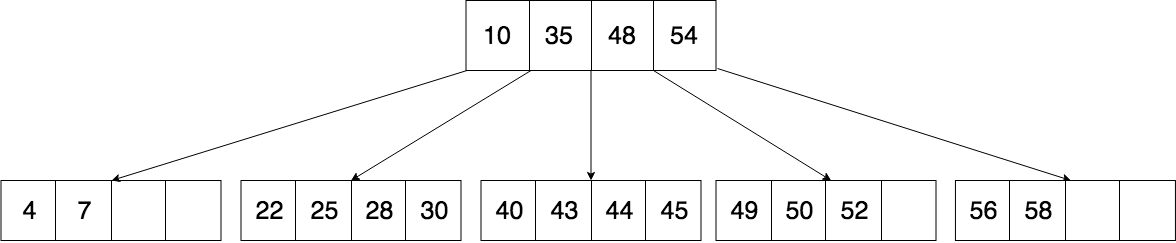
\includegraphics[scale=0.3]{figures/ExampleBTree.png}
    \caption{Example \textbf{B-Tree} with 19 keys. $d = 2$.}
    \label{fig:exB-Tree}
\end{figure}

B+-Trees are a variant of B-Trees: a balanced search tree data structure. B-Trees were first introduced by Bayer and McCreight \cite{bayer1970organization} as a method for indexing records stored in files on secondary storage. Figure \ref{fig:exB-Tree} shows an example B-Tree. Each node in a B-Tree has an order $d$ that determines its capacity, i.e. how many keys it can hold. Each node, except the root, must have between $d$ and $2d$ keys. The root can have between $0$ and $2d$ keys. The pointer between two keys $a$ and $b$ contain keys whose values are greater than $a$ and smaller than $b$.

\begin{figure}[htbp]
    \centering
    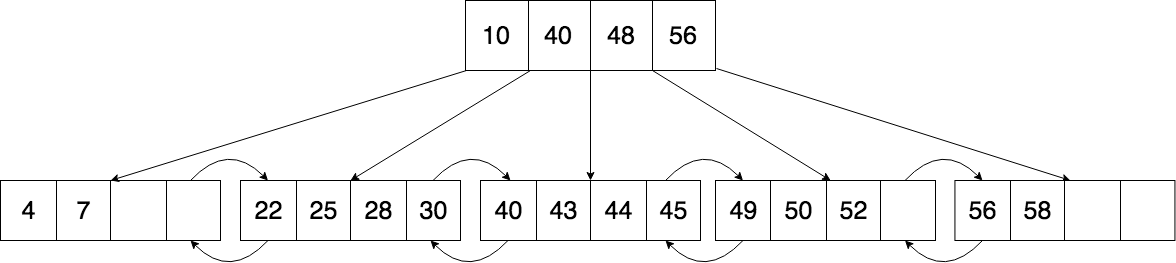
\includegraphics[scale=0.3]{figures/ExampleBplusTree.png}
    \caption{Example \textbf{B+-Tree} with 15 keys. $d = 2$.}
    \label{fig:exB+-Tree}
\end{figure}

B+-Trees vary from their B-Tree counterparts in that their nodes are divided into a \textit{sequence} and \textit{index} set. Figure \ref{fig:exB+-Tree} shows a simple B+-Tree with one internal node (the root) and five leaf nodes holding the keys stored in the tree. The sequence set consists of the leaves of the B-Tree. The index set consists of the internal (non-leaf) nodes. So record keys are found in the leaves, while the internal node contain copies of keys that guide searches to the leaf node containing the desired record. These copies are the result of node splitting. A node split occurs when we try to insert a new key into a full node in order to make room for the new key. After a node split, a copy of the first key in the newly created second node and a pointer to the second node is pushed into the parent node of the first node. This process continues if the parent node is full. Furthermore, traditional B+-Trees have cross-links between leaves. This means the sequence set forms a (doubly) linked list. Restricting keys / records to the leaves leads to simpler deletion and enables fast sequential access of keys. Getting the next key in the sequence of current keys always takes constant time. A survey of B-Trees and their variants, including B+-Trees, was presented by Comer in \cite{comer1979ubiquitous}. 

\subsection{Handling Variable-length Keys} \label{sec:VarLCPKeysMasstree}

\subsubsection{Variable-length Keys and Keys with Long Common Prefixes}

B+-Trees are an excellent data structure for record insertions, updates and retrieval. Any record in a B+-Tree containing a large number of records can be accessed with a few node accesses. Indeed the number of node accesses involved in an operation is a good cost model when analyzing the performance of file-based databases and even main-memory databases. However, it pays to consider the cost of string compares in B+-Trees in the presence of variable length keys that could possibly share long common prefixes. This is because aside from node accesses a fair amount of time is spent looking for the appropriate key in an internal node (to guide search) or in a leaf node (to retrieve the desired record), when searching for a record. The time spent comparing strings is more significant in main-memory databases where the cost of node accesses is relatively low compared to file-based databases.

\begin{figure}[htbp]
    \centering
    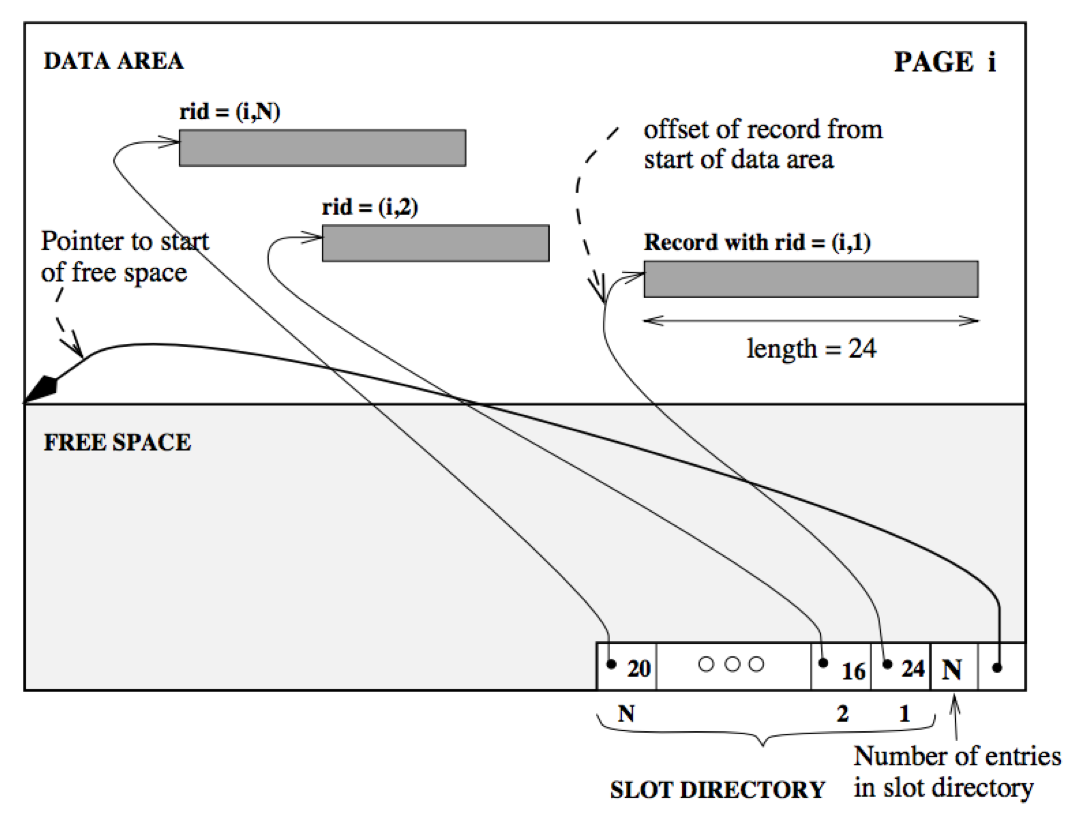
\includegraphics[scale=0.4]{figures/pagevariablelengthkeys.png}
    \caption{Example B+-Tree with $d = 2$.}
    \label{fig:exNodePageB+-Tree}
\end{figure}

Most B+-Tree implementations handle variable-length keys by adding an extra level of indirection. A page/node containing variable length keys in a file-based B+-Tree will look something like Figure \ref{fig:exNodePageB+-Tree} (from page 220 of \cite{ramakrishnan2000database}). VoltDB (a main memory database) also adds a level of indirection when storing long record fields. Figure \ref{fig:voltDBStructure} (from page 48 of \cite{main-mem-dbs}) shows how records are stored in VoltDB's storage layer. Here, record tuples are stored in fixed-sized blocks. If a tuple's field is greater than 8 bytes, it is stored in a variable-size block; the memory address of the item is then stored in the field's location in the tuple instead. In both of the presented cases,  there is a level of indirection involved in finding desired keys within a node. Aside from this being less cache friendly, there is the added complication of maintaining the free area within a node page. Moreover, it is possible that some space could be wasted due to fragmentation within a data page.


\begin{figure}[hbtp]
    \centering
    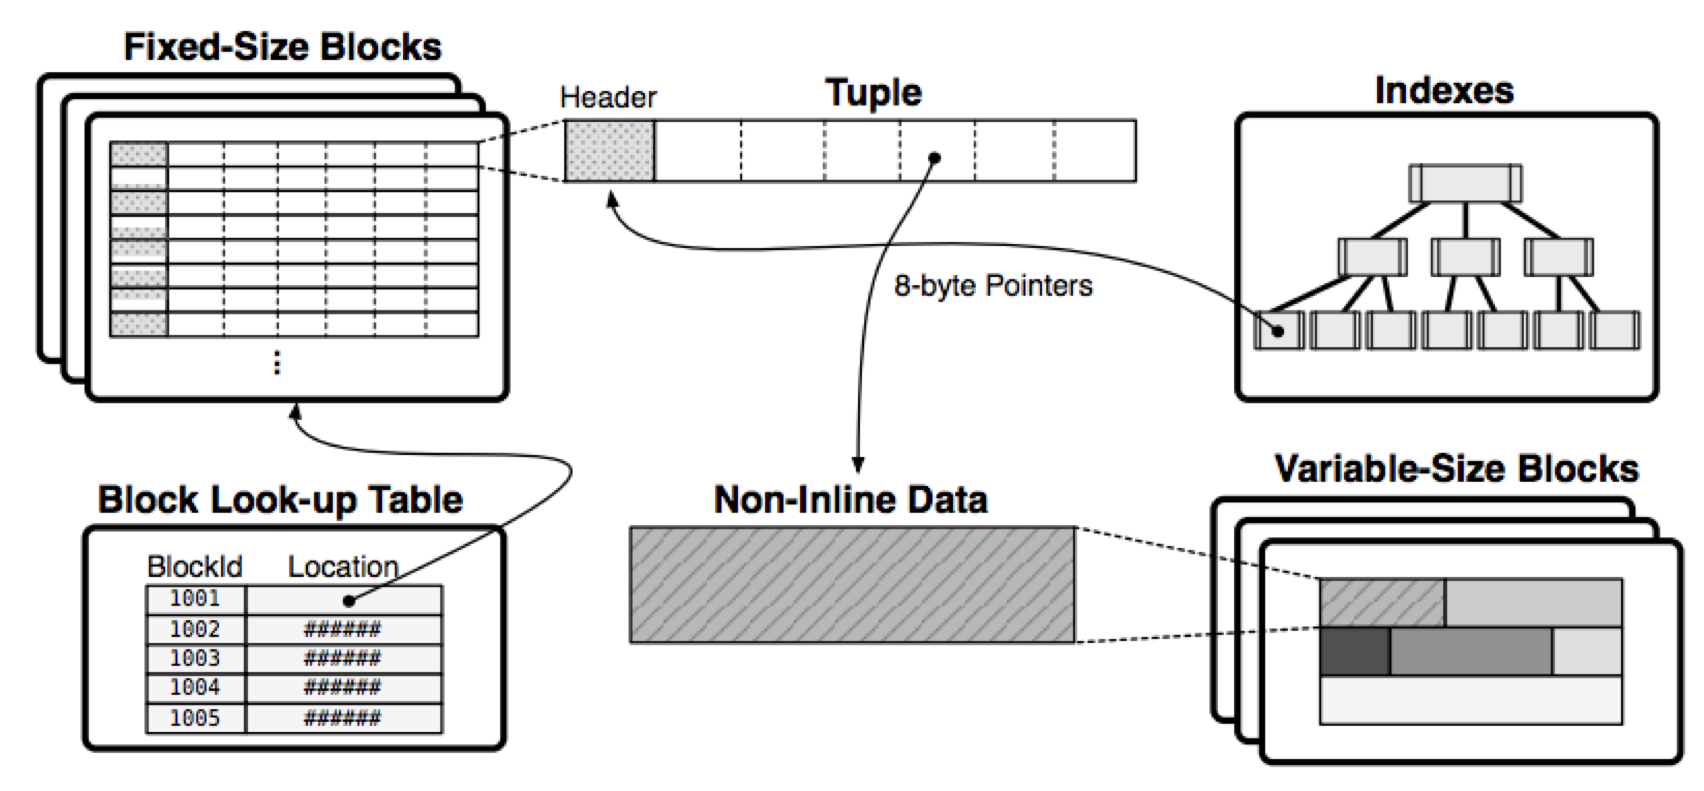
\includegraphics[scale=0.4]{figures/voltdbvariablelengthkey.png}
    \caption{VoltDB storage layout.}
    \label{fig:voltDBStructure}
\end{figure}

\begin{comment}
 VoltDB/H-Store (a main memory database)\cite{main-mem-dbs}, for example, has a fixed-size block pool containing table tuples. If a field is larger than 8-bytes, it is stored in a variable-length block instead. The field in the tuple contains the address of the block instead of the 8-byte data. Traditional file based databases use an "indirection vector"\cite{graefe2011modern} or "directory of slots"\cite{ramakrishnan2000database} with elements of fixed size that point to records in a data area in the page. Each page is a node in the B-Tree. Our implementation follows MassTree's approach instead of the standard approach. An overview of MassTree's datastructure is given below.
\end{comment}
 

\begin{table}[h]
\centering
\label{tab:exampleResourceURLTable}
\begin{tabular}{|l|c|}
\hline
Resource URL                & \multicolumn{1}{l|}{Unique Clients} \\ \hline \hline
/apis/v1/photos/albums      & 753                        \\ \hline
/apis/v1/photos/profile     & 486                        \\ \hline
/apis/v1/info/tutorial      & 1000                       \\ \hline
/apis/v1/info/preferences   & 1000                       \\ \hline
\end{tabular}
\caption{Example of HTTP resource URLs and unique client counts.}
\end{table}

B+-Trees can also run into issues with keys with long prefixes. Consider a web server that periodically processes it server logs and stores in a databases resources requested and the count of how many unique clients requested that resource. An example database table is shown in Table \ref{tab:exampleResourceURLTable}. The corresponding primary B+-Tree index on resource URLs would look like the B+-Tree shown in Figure \ref{fig:urlExampleB+-Tree} (only keys are shown). This simple example is illustrative of how B+-Trees handle long keys that possibly have long common prefixes. Space is wasted saving copies of long keys and performance falls. This is because when searching for any key in the tree, more character comparisons have to be made to determine the lexicographical relationship between two strings that share a long common prefix. 

\begin{figure}[h]
    \centering
    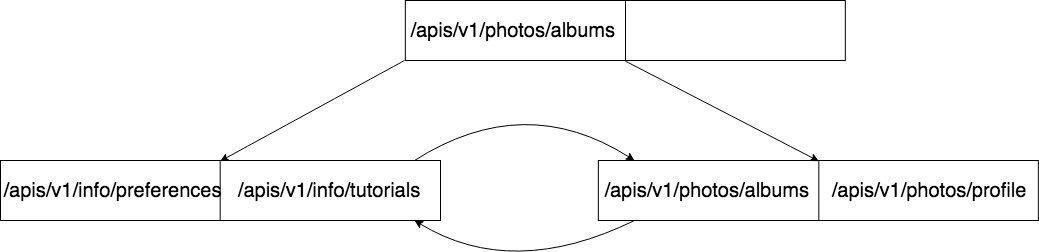
\includegraphics[scale=0.3]{figures/urlexamplebtree.png}
    \caption{B+-Tree index of Table \ref{tab:exampleResourceURLTable} (only keys are shown).}
    \label{fig:urlExampleB+-Tree}
\end{figure}

For the simple example in Table \ref{tab:exampleResourceURLTable}, these issues are not a cause for concern. However, one could imagine a much larger table where there are millions of rows where most keys share long common prefixes. These issues would be intolerable. Even if we take the prefix B+-Tree approach (see \cite{comer1979ubiquitous,ramakrishnan2000database}) - where instead of storing copies of keys in internal nodes, the smallest possible delimiter is used - space could still be wasted if there the common prefixes are long. In Figure \ref{fig:urlExamplePrefixB+-Tree} we see that the root of the prefix B+-Tree index of Table \ref{tab:exampleResourceURLTable} contains the delimiter key \say{/apis/v1/p}. If the largest key to the left of the root and the smallest key to the right of the root shared a longer common prefix, then delimiter key must be longer.


\begin{figure}[h]
    \centering
    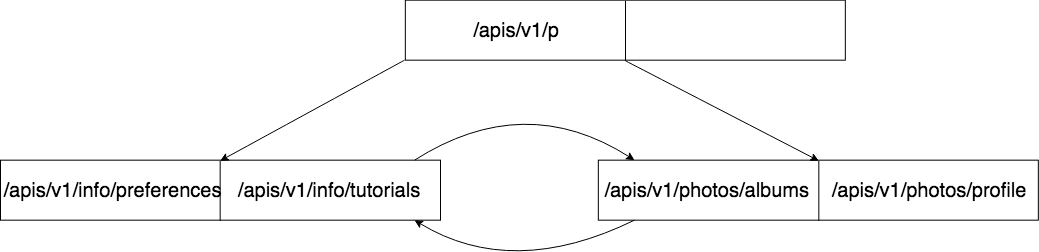
\includegraphics[scale=0.3]{figures/urlexampleprefixbtree.png}
    \caption{Prefix B+-Tree index of Table \ref{tab:exampleResourceURLTable} (only keys are shown).}
    \label{fig:urlExamplePrefixB+-Tree}
\end{figure}


\subsubsection{The solution: Masstree}

Given the aforementioned challenges, our key-value store is based on the Masstree system / data structure. This is to ensure our key-value store can properly handle variable length keys and keys sharing long common prefixes,. 

Masstree \cite{masstree} is an in-memory network key-value storage server that supports range queries. It is also the name of the data structure that the server uses to store key-value pairs. The Masstree data structure is designed to efficiently support arbitrary-length keys, including keys with long common prefixes.  The Masstree system supports \texttt{$get_c(k)$}, \texttt{$put_c(k,v)$}, \texttt{$remove(k)$} and \texttt{$getrange_c(k,n)$} operations. As one might expect, \texttt{get} returns the value associated with a key \texttt{k}. \texttt{put} adds a key-value pair \texttt{(k,v)} into the key-value store or updates the value (\texttt{v}) associated with a key \texttt{k}. \texttt{getrange} returns up to the first \texttt{n} key-value pairs greater than or equal to \texttt{k} in the database. Finally the parameter c is a list of column numbers that allow a client to get or set portions of a key's value. 

The authors of \cite{masstree} describe the Masstree data structure as a \say{trie-like concatenation of B+-Trees}. The structure of a Masstree tree is shown in Figure \ref{fig:MasstreeTreeStructure}. The tree has multiple layers containing one or more B+-Tree. The root layer contains at most one B+-Tree, the second layer contains at most $2^{64}$ trees - one for every possible key the first layer can have - and so on. Each B+-Tree and layer is responsible for some 8-byte slice of a key. Masstree's B+-Trees consist of interior nodes and border nodes(see Figure \ref{fig:MasstreenodeDS}). 

\begin{figure}[htbp]
    \centering
    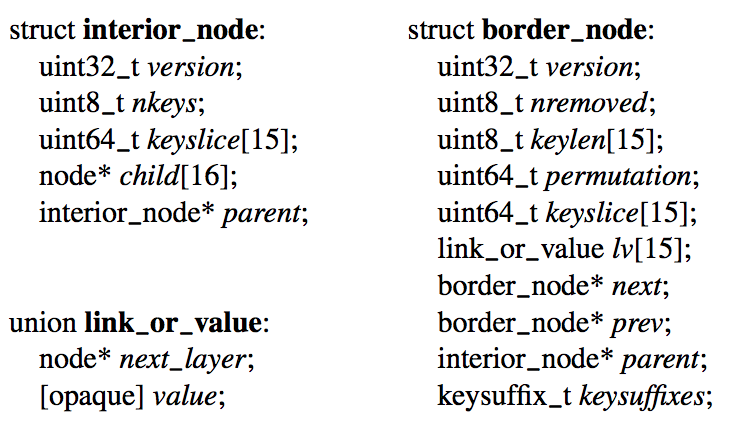
\includegraphics[scale=0.50]{figures/masstreenodestructures.png}
    \caption{Masstree Node Data Structures \cite{masstree}}
    \label{fig:MasstreenodeDS}
\end{figure}

Border nodes are similar to traditional B+-Tree leaf nodes. They have cross-links (to aid the \texttt{getrange} operation), keys and key values. However, Masstree's border nodes are unique in that their keys are identified by an 8-byte key slice and a key length. This means that a single Masstree B+-Tree can represent multiple (at most 10) keys with each key slice. At most 9 different keys for every possible prefix of the keyslice (keys with length 0 to length 8) and a 10th key in the event that there is a key suffix or a link to the next layer. Not all key slices can have 10 different keys. A key slice with no null bytes can have only two different keys. A key with a null byte at the end can have three different keys. Moreover, for each key in a border node, there is a value or a link to a B+-Tree in the next layer. Whether a key points to a value or another B+-Tree depends on the value of its key length field. If a key's key length is greater than 8, then the key has a suffix and a value or has a link to another layer instead of a value. 

\begin{figure}[hbtp]
    \centering
    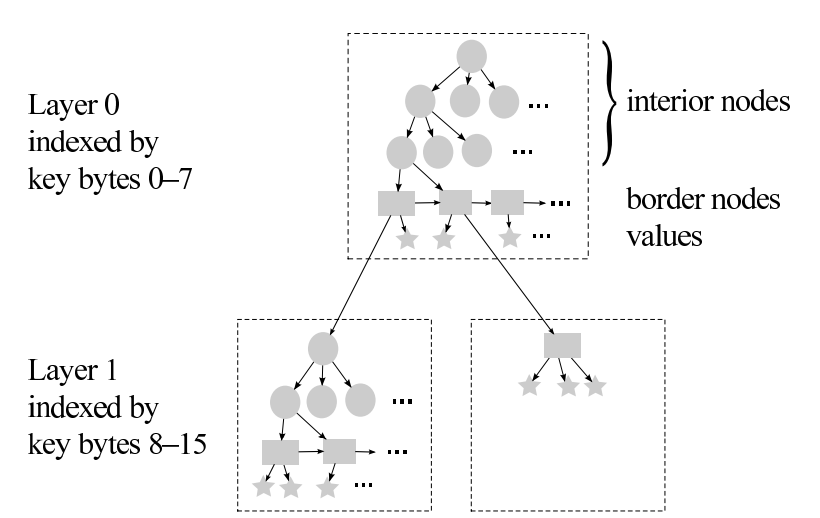
\includegraphics[scale=0.50]{figures/masstreedatastructure.png}
    \caption{Masstree Tree Structure \cite{masstree}}
    \label{fig:MasstreeTreeStructure}
\end{figure}

MassTree border nodes also contain keysuffix data structures in the event that a key's suffixes aren't shared by any other keys with the same prefix. That is, if we have the keys \texttt{"AB"} and \texttt{"ABCDEFGH!"} in our key-value store, there is no need to create a second layer to index the last byte of the second key. On the contrary, we store \texttt{"AB"} (2 bytes) and \texttt{"ABCDEFGH!"} (9 bytes) with their appropriate key slices and key lengths in a B+-Tree with a single node (layer 0). Then we set the keysuffix for the latter of the key slices to be \texttt{"!"}. However, if we have another key \texttt{"ABCDEFGH*"}, key slice \texttt{"ABCDEFGH"} must now point to a new layer. In addition, the string whose suffix is $"!"$ is inserted in the new layer with its original value and the new string whose suffix is \texttt{"*"} is inserted in the new layer with its value. Generally, if a key is $8h$ bytes long, its value will be stored at layer $x$ where $x < h$. So, if a key is 8 bytes or less, its value will be referenced by a keyslice in the root layer's B+-Tree. If a key is 40 bytes long, its value will be stored in one of layers 0 to 4. This is because key suffixes can be stored in a bordernode, if no other prefixes of the full key share in the keyslices up to a layer and part of the suffix. The keysuffix data structure means that unnecessary layers are not created when there are many relatively long keys that do not share common prefixes. On the other hand, if there are long keys that share common prefixes, then multiple layers (relatively small layers) would be responsible for a portion of the common prefix. Which keeps retrievals fast as shown in the Evaluation Section \ref{sec:Evaluation}.

\begin{comment}
Operations in MassTree can benefit from cache-locality compared to typical B+-Tree schemes where variable length keys are handled by an extra level of indirection (areas outside the tree to store long keys) (reference???). Operations also benefit by reducing space costs associated with storing multiple keys with common prefixes separately.
\end{comment}
